\section{Introduction}
\label{sec:introduction}

A slicer turns a part into machine motion, and on the way it makes several decisions: which source to traverse, in what order, how to place it in the part, how to turn the tool path into machine motion, and how that motion deposits material. Most slicers bundle these decisions into one algorithm, so two slicers differ in several decisions at once, and a limit that many of them share can go unnoticed because it lies in a decision that none of them varies. Separating the decisions lets slicers be compared one decision at a time, lets each guarantee and failure be traced to the decision that supplies it, and lets alternatives be constructed by making one decision differently. This paper develops that separation as a framework, the map chain, and demonstrates it on interruptions.

The motion a slicer produces is rarely one continuous stroke. The flow stops between layers, and a robot may have to change posture partway through. Some of these interruptions are chosen by a planner and could be planned away; others are forced by the structure of the slicer. We use the framework to find which stage forces them and how to design a slicer that avoids them. Figure~\ref{fig:teaser} shows a tool path built this way.

\begin{figure}[!ht]
  \centering
  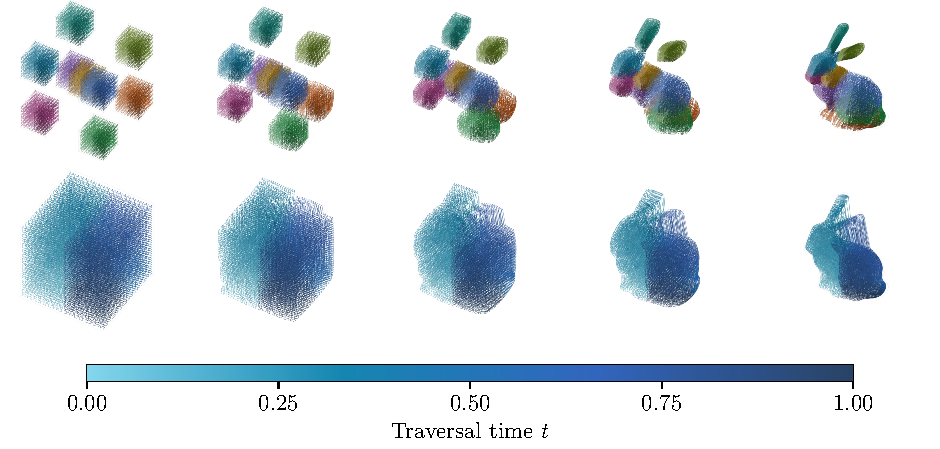
\includegraphics[width=\textwidth]{figures/bunny_transport_decomposition.pdf}
  \caption{The first application of the framework: a connected volume, not a stack of layers, as the source. Top: a decomposed source of nine cubes, each transported onto one piece of the Stanford bunny; each piece has its own colour, light at its start and dark at its end. Bottom: a Hilbert path through one cube ($32\,768$ cells) is moved into the bunny by optimal transport, coloured by traversal time. Intermediate shapes are drawn for illustration. The visiting order comes from the cubes, and the shape, including the ears, from the map alone.}
  \label{fig:teaser}
\end{figure}

On a simple cylinder, a layered raster must stop between layers, and the count roughly doubles each time the resolution doubles (Section~\ref{main:evidence}). Each stop of the material flow can leave a seam, and in some processes a stop is especially costly: it can cut reinforcing fibre in continuous-fibre printing \cite{fang2024exceptional}, cause a restart defect in wire-arc deposition \cite{ding2014toolpath}, or weaken the bond in concrete printing \cite{tay2019timegap}. Better paths within each layer remove some stops, but not those between layers. A robot shows the same pattern one stage later: when obstacles split its safe postures into separate families, some tool paths cannot be followed without a posture reset, however good the inverse kinematics.

\paragraph{The map-chain framework.}
We treat a slicer as a chain of maps, from a source representation through the part and the machine to the built part (Section~\ref{main:chain}). The framework makes three contributions: (i)~a common description for comparing slicers, in which each slicer is a choice of links and of their construction order, so that slicers can be compared link by link and their shared choices become visible (Section~\ref{main:families}); (ii)~composition rules, by which coverage, continuity, containment, and implementation error compose from link to link, so that each guarantee or failure can be traced to the link that supplies it (Section~\ref{main:compose}); and (iii)~a design procedure, in which replacing a link choice that existing slicers hold fixed, or changing the construction order, defines a new construction whose surviving guarantees and new obligations the rules state. Forced interruptions are topological, because each continuous stretch of motion remains within one path component of the space it moves in: a plan that must visit $c$ components is interrupted at least $c-1$ times, and the chain locates the link that supplies the components (Section~\ref{main:source}). We demonstrate the procedure on two shared choices that, in the slicing literature we review, force interruptions at two different links; the resulting constructions show what the framework makes visible, not its full extent.

\paragraph{First application: changing the source.}
Every reviewed solid-filling slicer traverses a source of separate layers or surfaces. Separating the source from the traversal makes the alternative visible: one connected volume, traversed directly. The \emph{transported Hilbert path} (Section~\ref{main:construction}) orders a cube with a three-dimensional Hilbert curve and carries it into the part by optimal transport, so that the traversal fixes the visiting order and the geometry map the shape. On convex parts the path is continuous and has exactly the prescribed occupation measure; on non-convex parts, decomposing the source into near-convex pieces meets containment up to each piece's hull gap.

\paragraph{Second application: changing the construction order.}
Every reviewed slicer builds the tool path first, and that path then fixes how often the robot must switch between families of safe postures. Separating the geometry map from the lift makes the alternative visible: build admissible machine motion first and derive the tool path from it through forward kinematics. This requires a new map from the source into configurations. In \emph{kinematics-first slicing} (Section~\ref{main:next}), guarantees and obligations trade places: static feasibility holds by construction, while coverage and the prescribed deposition density become obligations, met by a source split that the posture families guide.

\paragraph{Scope.}
All evidence is computational. The volumetric experiments end at the geometric tool path, and no part has been printed. In the robot experiment, feasibility is static, and the separation of posture families and the optimality of the switch counts hold only in a sampled model. Physical posture resets and material deposition are not modelled. Section~\ref{main:outlook} returns to these boundaries.

\paragraph{Research prototype and reproducibility.}
The research prototype, saved reference results, and figure-generation code are available at \url{https://github.com/pobol2/Topology-of-Slicing}.
